\documentclass[11pt,a4paper]{article}
\usepackage[T1]{fontenc}
\usepackage{algorithmicx}
\usepackage{algorithm}
\usepackage{algpseudocode}
\usepackage{amssymb}
\usepackage{graphicx}
\usepackage{hyphenat}
\usepackage{isabelle}
\usepackage{isabellesym}
\usepackage{subfig}
\usepackage{tikz}
\usepackage{todonotes}
\usepackage{mathtools}
\usepackage{csquotes}
\usepackage{authblk}

\usetikzlibrary{positioning}

% further packages required for unusual symbols (see also
% isabellesym.sty), use only when needed

%for \<leadsto>, \<box>, \<diamond>, \<sqsupset>, \<mho>, \<Join>,
  %\<lhd>, \<lesssim>, \<greatersim>, \<lessapprox>, \<greaterapprox>,
  %\<triangleq>, \<yen>, \<lozenge>

%\usepackage{eurosym}
  %for \<euro>

%\usepackage[only,bigsqcap]{stmaryrd}
  %for \<Sqinter>

%\usepackage{eufrak}
  %for \<AA> ... \<ZZ>, \<aa> ... \<zz> (also included in amssymb)

%\usepackage{textcomp}
  %for \<onequarter>, \<onehalf>, \<threequarters>, \<degree>, \<cent>,
  %\<currency>

% This should be the last package used.
\usepackage{pdfsetup}

% URLs in roman style, theory text in math-similar italics.
\urlstyle{rm}
\isabellestyle{it}

% For uniform font size.
%\renewcommand{\isastyle}{\isastyleminor}

\begin{document}

\title{Strong Eventual Consistency of the Collaborative Editing Framework WOOT}
\author{Emin Karayel}
\author{Edgar Gonzàlez}
\affil{Google, Mountain View}
\maketitle

% Sane default for proof documents.
% \parindent 0pt\parskip 0.5ex
\setlength\parindent{1em}
\setlength\parskip{0.5ex}

\begin{abstract}
  Commutative Replicated Data Types (CRDTs) are a promising new class of data structures for large-scale shared mutable content in applications that only require eventual consistency.
The WithOut Operational Transforms (WOOT) framework is a CRDT for collaborative text editing introduced by Oster et al. (CSCW 2006) for which the eventual consistency property was verified only for a bounded model to date.
We contribute a formal proof for WOOTs strong eventual consistency.
\end{abstract}

\tableofcontents

\section{Introduction}%
A \emph{Replicated (Abstract) Data Type (RDT)} consists of ``\emph{multiple copies of a shared Abstract Data Type (ADT) replicated over distributed sites, [which] provides a set of primitive operation types corresponding to that of normal ADTs, concealing details for consistency maintenance}''~\cite{roh2009optimistic}.
RDTs can be classified as \emph{state-based} or \emph{operation-based} depending on whether full states (e.g., a document's text) or only the operations performed on them (e.g., character insertions and deletions) are exchanged among replicas.
Operation-based RDTs are \emph{commutative} when the integration of any two concurrent operations on any reachable replica state commutes~\cite{shapiro2011conflict}.

Commutative (Operation-Based) Replicated Data Types (CRDTs\footnote{Note that other authors like Shapiro et al.~\cite{shapiro2011conflict} use CmRDT to refer to Commutative RDTs, with CRDT standing for \emph{Conflict-free RDTs}.} from now on) enable sharing mutable content with optimistic replication---ensu\-ring high\hyp{}availability, responsive interaction, and eventual consistency without consensus\hyp{}ba\-sed concurrency control~\cite{letia2010consistency}.
They are used in highly scalable robust distributed applications~\cite{weiss2009logoot,brown2014riak}.

An RDT is \emph{eventually consistent} when, if after some point in time no further updates are made at any replica, all replicas eventually converge to equivalent states.
It is \emph{strongly eventually consistent} when it is eventually consistent and, whenever any two peers have seen the same set of updates (in possibly different order), they reach equivalent states immediately~\cite{shapiro2011conflict}.

The WithOut Operational Transforms (WOOT) Framework~\cite{oster2006data} was the first proposed CRDT for collaborative text editing~\cite{Briot2016}.
It has been implemented as part of several OSS projects~\cite{dallaway2016wootjs,emanouilov2016woot,kaplan2016woot,olson2016woot}.
However, the eventual consistency of WOOT has only been verified for a bounded model~\cite{oster2006data, oster2005real}.
A formal proof of WOOTs consistency can rigorously establish that there is no complex counter-example not identified by model checking.

The contribution of this work is one such proof that the WOOT Framework is strongly eventually consistent.
Its central idea is the association of a value from a dense totally ordered space to each inserted (and potentially deleted) character, using a recursive definition with respect to the acyclic graph induced by the predecessor and successor relation of the characters.
We then show that the strings in each peer remain sorted with respect to that value, i.e., that the values form a sort key for W-characters.\footnote{Note that the values themselves do not have to be actually computed, during the execution of the framework. Their existence and compatibility with the integration algorithm forms a witness for the consistency proof we are presenting.}
This resolves the conjecture posed by Oster et al.~\cite[conjecture 1]{oster2005real} and is also the key lemma to establish that the WOOT Framework has the strong eventual consistency property.

After reviewing related work in the following section, we formalize the WOOT Framework as a distributed application in Section~\ref{sec:wootFramework}.
We follow with the complete eventual consistency proof in Section~\ref{sec:proof} and summarize the established results in Section~\ref{sec:strong_eventual_consistency}. In Section~\ref{sec:proof_outline} we given overview of the proof
and follow up with a conrete formalized example in Section~\ref{sec:example}.

The presentation is structured such that all the definitions necessary to review the established results in Section~\ref{sec:strong_eventual_consistency} are part of Section~\ref{sec:wootFramework}.
This means it is possible to skip Section~\ref{sec:proof} entirely.

\section{Related Work}%
\label{sec:relatedWork}%
The first collaborative text editing tools were based on operational transformations (OT), and introduced by Ellis and Gibbs~\cite{ellis1989concurrency}.
The basic idea behind OT-based frameworks is to adjust edit operations, based on the effects of previously executed concurrent operations.
For instance, in Figure~\ref{fig:otDrawing}, peer B can execute the message received from peer A without correction, but peer A needs to transform the one received from peer B to reach the same state.

Proving the correctness of OT-based frameworks is error-prone and requires complicated case coverage~\cite{li2010admissibility,molli2006tombstone}.
Counter-examples have been found in most OT algorithms~\cite{roh2009optimistic}\cite[section 8.2]{gomes2017verifying}.

\begin{figure}[t]
\centering
\subfloat[Transformation-based]{\label{fig:otDrawing}%
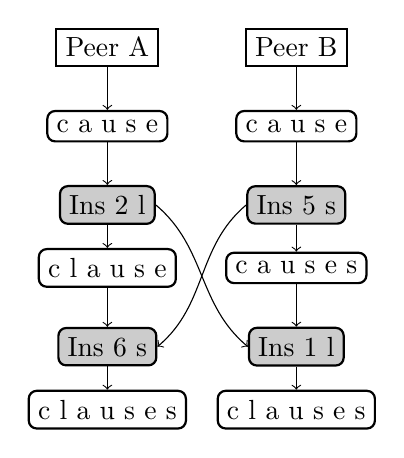
\begin{tikzpicture}[
  peernode/.style={rectangle, draw=black, thick},
  editnode/.style={rectangle, draw=black, fill=black!20, thick,rounded corners=.1cm},
  statenode/.style={rectangle, draw=black, thick,rounded corners=.1cm},
]
% Nodes.
\node[peernode] (peerA) at (0, 4.6) {Peer A};
\node[peernode] (peerB) at (2.4, 4.6) {Peer B};
\node[statenode] (stateA1) at (0, 3.6) {c a u s e};
\node[statenode] (stateB1) at (2.4, 3.6) {c a u s e};
\node[editnode] (editA1) at (0, 2.6) {Ins 2 l};
\node[editnode] (editB1) at (2.4, 2.6) {Ins 5 s};
\node[statenode] (stateA2) at (0, 1.8) {c l a u s e};
\node[statenode] (stateB2) at (2.4, 1.8) {c a u s e s};
\node[editnode] (editA2) at (0, 0.8) {Ins 6 s};
\node[editnode] (editB2) at (2.4, 0.8) {Ins 1 l};
\node[statenode] (stateA3) at (0, 0) {c l a u s e s};
\node[statenode] (stateB3) at (2.4, 0) {c l a u s e s};
% Lines.
\draw[->] (peerA.south) -- (stateA1.north);
\draw[->] (peerB.south) -- (stateB1.north);
\draw[->] (stateA1.south) -- (editA1.north);
\draw[->] (stateB1.south) -- (editB1.north);
\draw[->] (editA1.south) -- (stateA2.north);
\draw[->] (editB1.south) -- (stateB2.north);
\draw[->] (stateA2.south) -- (editA2.north);
\draw[->] (stateB2.south) -- (editB2.north);
\draw[->] (editA2.south) -- (stateA3.north);
\draw[->] (editB2.south) -- (stateB3.north);
\draw[->] (editA1.east) to[out=-40,in=140] (editB2.west);
\draw[->] (editB1.west) to[out=220,in=40] (editA2.east);
\end{tikzpicture}}
\hspace{0.5em}\vline\hspace{0.5em}%
\subfloat[Sort-key based]{\label{fig:crdtDrawing}%
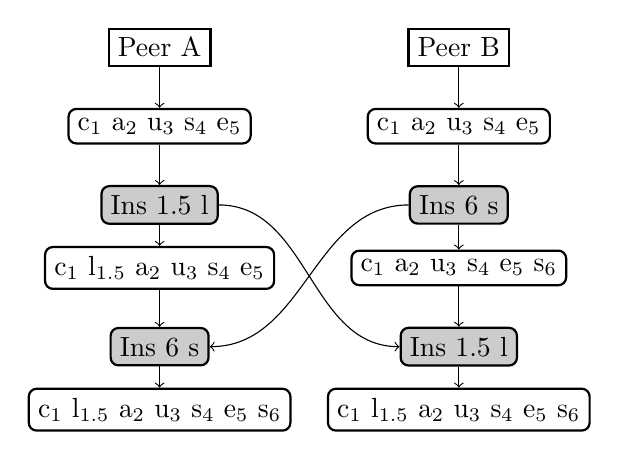
\begin{tikzpicture}[
  peernode/.style={rectangle, draw=black, thick},
  editnode/.style={rectangle, draw=black, fill=black!20, thick,rounded corners=.1cm},
  statenode/.style={rectangle, draw=black, thick,rounded corners=.1cm},
]
% Nodes. 5.5 - 1.7 = 4.5 - 0.7
\node[peernode] (peerA) at (0, 4.6) {Peer A};
\node[peernode] (peerB) at (3.8, 4.6) {Peer B};
\node[statenode] (stateA1) at (0, 3.6) {$\textrm{c}_1$ $\textrm{a}_2$ $\textrm{u}_3$ $\textrm{s}_4$ $\textrm{e}_5$};
\node[statenode] (stateB1) at (3.8, 3.6) {$\textrm{c}_1$ $\textrm{a}_2$ $\textrm{u}_3$ $\textrm{s}_4$ $\textrm{e}_5$};
\node[editnode] (editA1) at (0, 2.6) {Ins 1.5 l};
\node[editnode] (editB1) at (3.8, 2.6) {Ins 6 s};
\node[statenode] (stateA2) at (0, 1.8) {$\textrm{c}_1$ $\textrm{l}_{1.5}$ $\textrm{a}_2$ $\textrm{u}_3$ $\textrm{s}_4$ $\textrm{e}_5$};
\node[statenode] (stateB2) at (3.8, 1.8) {$\textrm{c}_1$ $\textrm{a}_2$ $\textrm{u}_3$ $\textrm{s}_4$ $\textrm{e}_5$ $\textrm{s}_6$};
\node[editnode] (editA2) at (0, 0.8) {Ins 6 s};
\node[editnode] (editB2) at (3.8, 0.8) {Ins 1.5 l};
\node[statenode] (stateA3) at (0, 0) {$\textrm{c}_1$ $\textrm{l}_{1.5}$ $\textrm{a}_2$ $\textrm{u}_3$ $\textrm{s}_4$ $\textrm{e}_5$ $\textrm{s}_{6}$};
\node[statenode] (stateB3) at (3.8, 0) {$\textrm{c}_1$ $\textrm{l}_{1.5}$ $\textrm{a}_2$ $\textrm{u}_3$ $\textrm{s}_4$ $\textrm{e}_5$ $\textrm{s}_{6}$};
% Lines.
\draw[->] (peerA.south) -- (stateA1.north);
\draw[->] (peerB.south) -- (stateB1.north);
\draw[->] (stateA1.south) -- (editA1.north);
\draw[->] (stateB1.south) -- (editB1.north);
\draw[->] (editA1.south) -- (stateA2.north);
\draw[->] (editB1.south) -- (stateB2.north);
\draw[->] (stateA2.south) -- (editA2.north);
\draw[->] (stateB2.south) -- (editB2.north);
\draw[->] (editA2.south) -- (stateA3.north);
\draw[->] (editB2.south) -- (stateB3.north);
\draw[->] (editA1.east) to[out=0,in=180] (editB2.west);
\draw[->] (editB1.west) to[out=180,in=0] (editA2.east);
\end{tikzpicture}}
\caption{Collaborative text editing}%
\end{figure}%

LSEQ~\cite{nedelec2013lseq}, LOGOOT~\cite{weiss2009logoot} and TreeDoc~\cite{preguica2009commutative} are CRDTs that create and send sort keys for symbols (e.g., $1.5$ and $6$ in Figure~\ref{fig:crdtDrawing}).
These keys can then be directly used to order them, without requiring any transformations, and are drawn from a dense totally ordered space.
In the figure rational numbers were chosen for simplicity, but more commonly lexicographically ordered sequences are used.\footnote{In addition, peers draw sort keys from disjoint (but dense) subsets to avoid concurrently choosing the same sort key.}
The consistency property of these frameworks can be established easily.
However, the space required per sort key potentially grows linearly with the count of edit operations.
In LSEQ, a randomized allocation strategy for new identifiers is used to reduce the key growth, based on empirically determined edit patterns---but in the worst-case the size of the keys will still grow linearly with the count of insert operations.
Preguica et al.~\cite{preguica2009commutative} propose a solution for this problem using regular rebalancing operations.
However, this can only be done using a consensus\hyp{}based mechanism, which is only possible when the number of participating peers is small.

A benefit of LSEQ, LOGOOT, and TreeDoc is that deleted symbols can be garbage-collected (though delete messages may have to be kept in a buffer if the corresponding insertion message has not arrived at a peer), in contrast to the WOOT Framework, where deleted symbols (tombstones) cannot be removed.

Replicated Growable Arrays (RGAs) are another data structure for collaborative editing, introduced by Roh et al.~\cite{roh2009optimistic}.
Contrary to the previous approaches, the identifiers associated to the symbols are not sort keys, but are instead ordered consistently with the happened-before relation.
A peer sends the identifier of the symbol immediately preceeding the new symbol at the time it was created and the actual identifier associated to the new symbol.
The integration algorithm starts by finding the preceeding symbol and skipping following symbols with a larger identifier before placing the new symbol.
The authors provide a mathematical eventual consistency proof. Recently, Gomes et. al.~\cite{gomes2017verifying} also formalized the eventual consistency property of RGAs using Isabelle/HOL.

In addition to the original design of WOOT by Oster et al.~\cite{oster2006data}, a number of extensions have also been proposed.
For instance, Weiss et al.~\cite{weiss2007wooki} propose a line-based version WOOTO, and Ahmed-Nacer et al.~\cite{nacer2011} introduce a second extension WOOTH which improves performance by using hash tables.
The latter compare their implementation in benchmarks against LOGOOT, RGA, and an OT algorithm.

To the best of our knowledge there are no publications that further expand on the correctness of the WOOT Framework.
The fact that the general convergence proof is missing is also mentioned by Kumawat and Khun\-teta~\cite[Section 3.10]{kumawat2010survey}.

% Generated text of all theories.
\input{session}

% Optional bibliography.
\bibliographystyle{abbrv}
\bibliography{root}

\end{document}

%%% Local Variables:
%%% mode: latex
%%% TeX-master: t
%%% End:
